\section{The blockchain}

A blockchain, seminal concept invented by Satoshi in 2009 [1], stores all information about all transactions that have taken place. When one knows all transactions, one also knows the current balance of each address. In Proof of Stake (POS) a node is randomly chosen among all nodes to add the next block to the blockchain. A block contains all transactions that have taken place in the network since the last block. The node adding this block adds a transaction sending newly minted Gridcoins to his personal wallet in proportion of the BOINC work he did. Other nodes accept the new block only if the transactions are all valid and if the newly minted Gridcoins claimed by the creator node correspond to the amount of BOINC work did by the creator node as written in a previously minted superblock. 

\begin{figure}
\centering
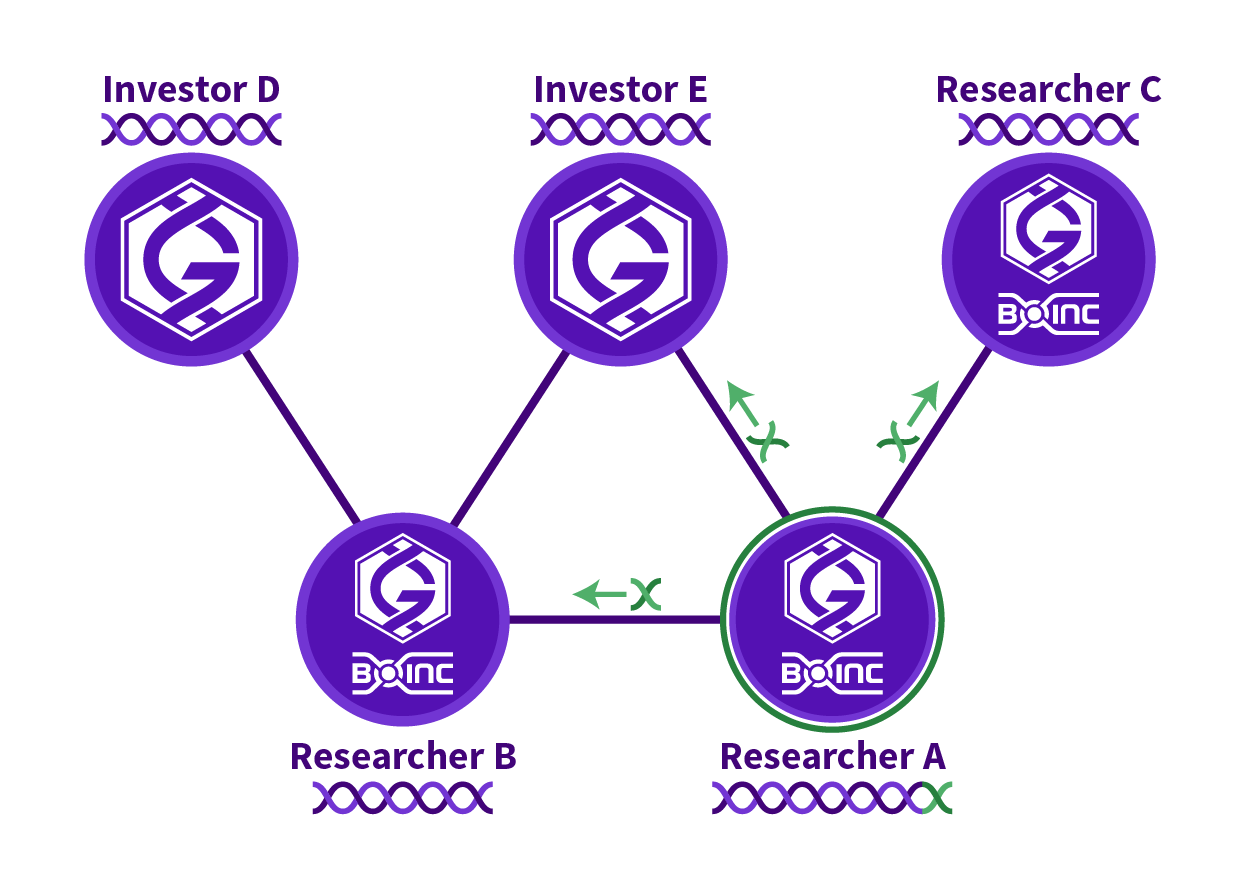
\includegraphics[scale=0.5]{figures/NetworkAndNodes_joshoeah}
\medskip
\caption{\textit{A researcher mines a new block and sends it to other node's blockchains, so that they verify it and incorporate it}}
\small
\end{figure}
 
When the probability is weighted by the current amount of Gridcoins, the reward that one gets on average for adding blocks is directly proportional to the amount of Gridcoins in possession (as this is the probability to be chosen to add the next block and get the reward) and thus can be seen as an interest for the user.
